% Three odd harmonics of a square wave. A picture of the idea, not a sum over zeros.
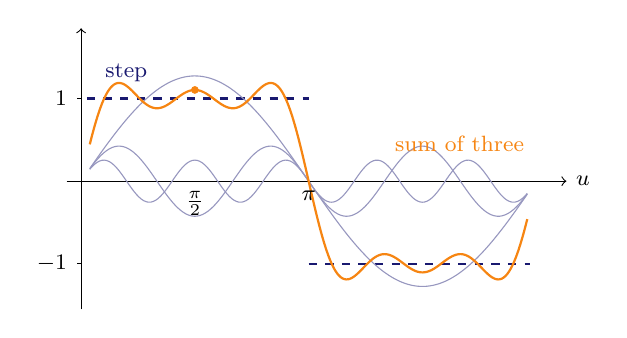
\begin{tikzpicture}[x=0.92cm,y=1.05cm,every node/.style={font=\footnotesize}]
  \draw[->] (-0.2,0)--(6.7,0) node[right] {$u$};
  \draw[->] (0,-1.55)--(0,1.85);
  \draw[MidnightBlue,dashed,thick] (0.08,1)--(3.1416,1);
  \draw[MidnightBlue,dashed,thick] (3.1416,-1)--(6.20,-1);
  \draw[MidnightBlue!45,domain=0.12:6.16,samples=140,smooth] plot (\x,{4/pi*sin(\x r)});
  \draw[MidnightBlue!45,domain=0.12:6.16,samples=160,smooth] plot (\x,{4/(3*pi)*sin(3*\x r)});
  \draw[MidnightBlue!45,domain=0.12:6.16,samples=180,smooth] plot (\x,{4/(5*pi)*sin(5*\x r)});
  \draw[BurntOrange,thick,domain=0.12:6.16,samples=240,smooth] plot (\x,{4/pi*(sin(\x r)+sin(3*\x r)/3+sin(5*\x r)/5)});
  \fill[BurntOrange] (1.5708,{52/(15*pi)}) circle (1.4pt);
  \node[MidnightBlue,anchor=south west] at (0.2,1.08) {step};
  \node[BurntOrange,anchor=west] at (4.2,0.45) {sum of three};
  \node[below] at (1.5708,0) {$\frac\pi2$};
  \node[below] at (3.1416,0) {$\pi$};
  \draw (0,1)--(-0.06,1) node[left] {$1$};
  \draw (0,-1)--(-0.06,-1) node[left] {$-1$};
\end{tikzpicture}
